\documentclass{article}

\usepackage{arxiv}

\usepackage[utf8]{inputenc} % allow utf-8 input
\usepackage[T1]{fontenc}    % use 8-bit T1 fonts
\usepackage{lmodern}        % https://github.com/rstudio/rticles/issues/343
\usepackage{hyperref}       % hyperlinks
\usepackage{url}            % simple URL typesetting
\usepackage{booktabs}       % professional-quality tables
\usepackage{amsfonts}       % blackboard math symbols
\usepackage{nicefrac}       % compact symbols for 1/2, etc.
\usepackage{microtype}      % microtypography
\usepackage{graphicx}

\title{Machine Learning Methods for Modeling and Classification of
fashion MNIST}

\author{
    David Blumenstiel
   \\
    Department of Data Science and Information Systems \\
    CUNY School of Professional Studies \\
  NY, NY 1001 \\
  \texttt{\href{mailto:blumenstieldavid@gmail.com}{\nolinkurl{blumenstieldavid@gmail.com}}} \\
   \And
    Bonnie Cooper
   \\
    Department of Biological Sciences \\
    SUNY College of Optometry \\
  NY, NY 10036 \\
  \texttt{\href{mailto:bcooper@sunyopt.edu}{\nolinkurl{bcooper@sunyopt.edu}}} \\
   \And
    Robert Welk
   \\
    Department of Data Science and Information Systems \\
    CUNY School of Professional Studies \\
  NY, NY 1001 \\
  \texttt{\href{mailto:robert.j.welk@gmail.com}{\nolinkurl{robert.j.welk@gmail.com}}} \\
   \And
    Leo Yi
   \\
    Department of Data Science and Information Systems \\
    CUNY School of Professional Studies \\
  NY, NY 1001 \\
  \texttt{\href{mailto:leo.yi35@spsmail.cuny.edu}{\nolinkurl{leo.yi35@spsmail.cuny.edu}}} \\
  }

\usepackage{color}
\usepackage{fancyvrb}
\newcommand{\VerbBar}{|}
\newcommand{\VERB}{\Verb[commandchars=\\\{\}]}
\DefineVerbatimEnvironment{Highlighting}{Verbatim}{commandchars=\\\{\}}
% Add ',fontsize=\small' for more characters per line
\usepackage{framed}
\definecolor{shadecolor}{RGB}{248,248,248}
\newenvironment{Shaded}{\begin{snugshade}}{\end{snugshade}}
\newcommand{\AlertTok}[1]{\textcolor[rgb]{0.94,0.16,0.16}{#1}}
\newcommand{\AnnotationTok}[1]{\textcolor[rgb]{0.56,0.35,0.01}{\textbf{\textit{#1}}}}
\newcommand{\AttributeTok}[1]{\textcolor[rgb]{0.77,0.63,0.00}{#1}}
\newcommand{\BaseNTok}[1]{\textcolor[rgb]{0.00,0.00,0.81}{#1}}
\newcommand{\BuiltInTok}[1]{#1}
\newcommand{\CharTok}[1]{\textcolor[rgb]{0.31,0.60,0.02}{#1}}
\newcommand{\CommentTok}[1]{\textcolor[rgb]{0.56,0.35,0.01}{\textit{#1}}}
\newcommand{\CommentVarTok}[1]{\textcolor[rgb]{0.56,0.35,0.01}{\textbf{\textit{#1}}}}
\newcommand{\ConstantTok}[1]{\textcolor[rgb]{0.00,0.00,0.00}{#1}}
\newcommand{\ControlFlowTok}[1]{\textcolor[rgb]{0.13,0.29,0.53}{\textbf{#1}}}
\newcommand{\DataTypeTok}[1]{\textcolor[rgb]{0.13,0.29,0.53}{#1}}
\newcommand{\DecValTok}[1]{\textcolor[rgb]{0.00,0.00,0.81}{#1}}
\newcommand{\DocumentationTok}[1]{\textcolor[rgb]{0.56,0.35,0.01}{\textbf{\textit{#1}}}}
\newcommand{\ErrorTok}[1]{\textcolor[rgb]{0.64,0.00,0.00}{\textbf{#1}}}
\newcommand{\ExtensionTok}[1]{#1}
\newcommand{\FloatTok}[1]{\textcolor[rgb]{0.00,0.00,0.81}{#1}}
\newcommand{\FunctionTok}[1]{\textcolor[rgb]{0.00,0.00,0.00}{#1}}
\newcommand{\ImportTok}[1]{#1}
\newcommand{\InformationTok}[1]{\textcolor[rgb]{0.56,0.35,0.01}{\textbf{\textit{#1}}}}
\newcommand{\KeywordTok}[1]{\textcolor[rgb]{0.13,0.29,0.53}{\textbf{#1}}}
\newcommand{\NormalTok}[1]{#1}
\newcommand{\OperatorTok}[1]{\textcolor[rgb]{0.81,0.36,0.00}{\textbf{#1}}}
\newcommand{\OtherTok}[1]{\textcolor[rgb]{0.56,0.35,0.01}{#1}}
\newcommand{\PreprocessorTok}[1]{\textcolor[rgb]{0.56,0.35,0.01}{\textit{#1}}}
\newcommand{\RegionMarkerTok}[1]{#1}
\newcommand{\SpecialCharTok}[1]{\textcolor[rgb]{0.00,0.00,0.00}{#1}}
\newcommand{\SpecialStringTok}[1]{\textcolor[rgb]{0.31,0.60,0.02}{#1}}
\newcommand{\StringTok}[1]{\textcolor[rgb]{0.31,0.60,0.02}{#1}}
\newcommand{\VariableTok}[1]{\textcolor[rgb]{0.00,0.00,0.00}{#1}}
\newcommand{\VerbatimStringTok}[1]{\textcolor[rgb]{0.31,0.60,0.02}{#1}}
\newcommand{\WarningTok}[1]{\textcolor[rgb]{0.56,0.35,0.01}{\textbf{\textit{#1}}}}

\usepackage{longtable,booktabs,array}
\usepackage{calc} % for calculating minipage widths
% Correct order of tables after \paragraph or \subparagraph
\usepackage{etoolbox}
\makeatletter
\patchcmd\longtable{\par}{\if@noskipsec\mbox{}\fi\par}{}{}
\makeatother
% Allow footnotes in longtable head/foot
\IfFileExists{footnotehyper.sty}{\usepackage{footnotehyper}}{\usepackage{footnote}}
\makesavenoteenv{longtable}

% Pandoc citation processing
\newlength{\csllabelwidth}
\setlength{\csllabelwidth}{3em}
\newlength{\cslhangindent}
\setlength{\cslhangindent}{1.5em}
% for Pandoc 2.8 to 2.10.1
\newenvironment{cslreferences}%
  {}%
  {\par}
% For Pandoc 2.11+
\newenvironment{CSLReferences}[2] % #1 hanging-ident, #2 entry spacing
 {% don't indent paragraphs
  \setlength{\parindent}{0pt}
  % turn on hanging indent if param 1 is 1
  \ifodd #1 \everypar{\setlength{\hangindent}{\cslhangindent}}\ignorespaces\fi
  % set entry spacing
  \ifnum #2 > 0
  \setlength{\parskip}{#2\baselineskip}
  \fi
 }%
 {}
\usepackage{calc} % for calculating minipage widths
\newcommand{\CSLBlock}[1]{#1\hfill\break}
\newcommand{\CSLLeftMargin}[1]{\parbox[t]{\csllabelwidth}{#1}}
\newcommand{\CSLRightInline}[1]{\parbox[t]{\linewidth - \csllabelwidth}{#1}\break}
\newcommand{\CSLIndent}[1]{\hspace{\cslhangindent}#1}



\begin{document}
\maketitle

\def\tightlist{}


\begin{abstract}
Fashion MNIST is a clothing classification dataset that is popular for
deep learning and computer vision applications. In this report, we use
Fashion MNIST to apply multiple machine learning methods reviewed in
Data622: Machine Learning and Big Data, an elective course for the
Masters of Science in Data Science at CUNY School of Professional
Studies. We explore approaches to reduce the dimensionality of the data
by engineering new descriptive features and performing Principal
Components Analysis. We then follow this up with machine learning
methods for classification such as Support Vector Machine and a
Convolutional Neural Network. We find that
\end{abstract}

\keywords{
    fashion MNIST
   \and
    machine learning
   \and
    classification
  }

\hypertarget{introduction}{%
\section{Introduction}\label{introduction}}

Fashion MNIST is a clothing classification dataset that builds in
complexity in comparison to the classic MNIST dataset. MNIST is a
dataset of handwritten digits that has been a go-to dataset for
benchmarking various image processing and machine learning algorithms
(LeCun et al. 1998). Classification algorithms applied to MNIST
revolutionized the field of image processing in the 90s (Krizhevsky,
Hinton, and others 2009). However, contemporary machine learning methods
can achieve 97\% accuracy. Convolutional neural nets score as high as
99.7\% accurate. As a result, MNIST is now considered too easy and, with
\textasciitilde48000 MNIST related publications (Noever and Noever
2021), MNIST has also been used exhaustively. Fashion MNIST was
developed as an alternative.

Fashion MNIST can serve as a direct drop-in replacement for MNIST.
Fashion MNIST and MNIST are both labeled data that share the same
dataset size: 60,000 training images and 10,000 test images.
Additionally, Fashion MNIST and MNIST images share the same dimensions
and structure: 10 distinct categories of grayscale images with 28x28
pixel size. Figure 1 depicts a sampling of several dozen example
Fashion-MNIST images. Due to the complexity and variety of the images,
Fashion MNIST is a more challenging dataset for machine learning
algorithms (Xiao, Rasul, and Vollgraf 2017).

\begin{figure}

{\centering 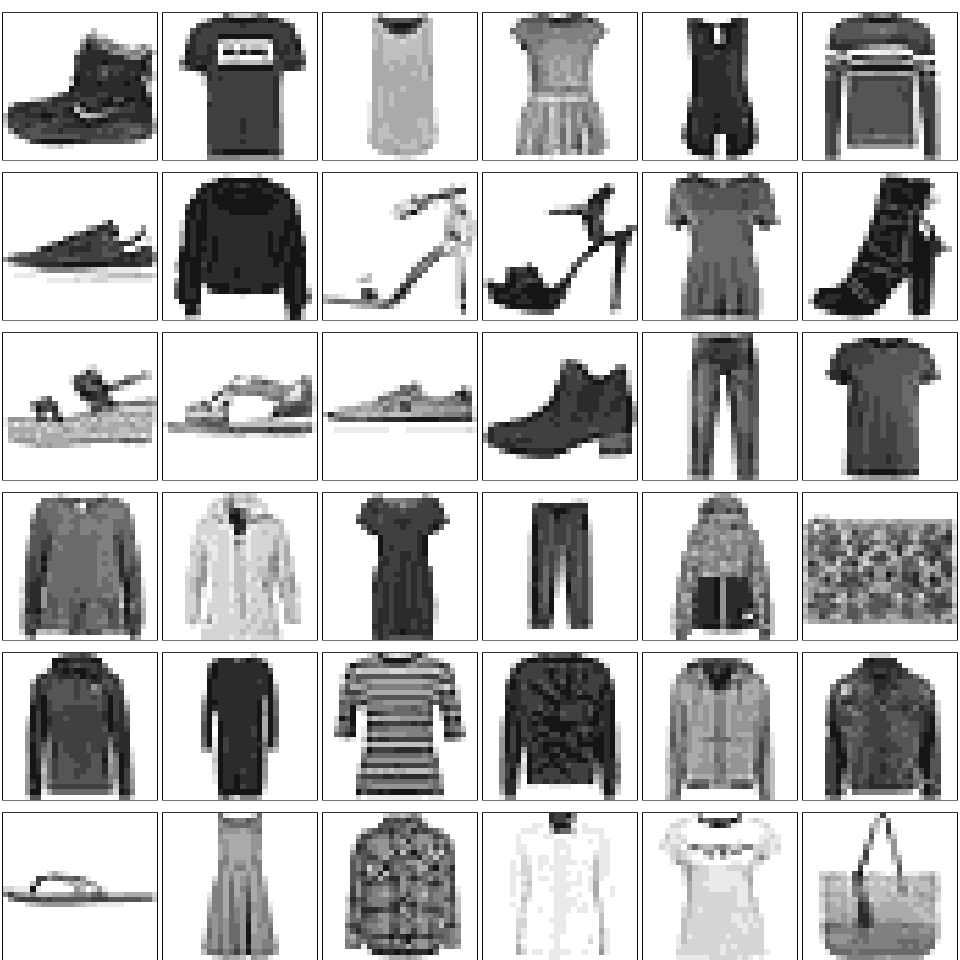
\includegraphics[width=0.6\linewidth]{/home/bonzilla/Documents/MSDS/Data622_group5_projects/FinalReport_Data622/exemplars} 

}

\caption{Exemplar Fashion-MNIST images. All image files are grayscale 28x28 images}\label{fig:unnamed-chunk-1}
\end{figure}

In this report we utilize Fashion MNIST to implement a variety of
machine learning approaches covered over the course of our studies in
Data622: Machine Learning and Big Data as part of the Masters of Data
Science program at CUNY School of Professional Studies. Our goal is to
optimize the classification of Fashion MNIST images using a variety of
machine learning algorithms. Here, we describe our approaches and
compare classification model performance.

With an image size of 28 x 28, Fashion MNIST images, in their raw form,
are very high dimensional data with a total of 784 features.
Additionally, there is a relatively high degree of correlation between
pixel values of a given image. That is to say that, unless an pixel is
at an object border, a light pixel in a region of the image is very
likely to be situated next to light neighboring pixels, likewise for
dark pixels. We can assess this by observing the mean and standard
deviation of the pixel values across the dataset.

Figure 2 visualizes the mean (left) and standard deviations (right) of
the pixel values for the \texttt{train} dataset. For both plots, higher
intensity values are rendered as dark whereas low values are light. For
many of the pixels in the image, the mean values is intermediate (gray)
whereas the standard deviation is relatively high (dark). These pixels
make up most of the variance in the dataset. However, we can see that
there are two regions of pixels towards the image center where the mean
pixel value is high (dark) while the pixel standard deviation is low
(light). For these regions, the pixels have consistently high pixel
values. Towards the periphery of the image there are pixels with both
low mean values (light) and low standard deviation (light). These pixels
have consistently low values. The pixels with either consistently low or
high values are of low information content and would not contribute much
to models for image classification if used as features. Therefore, we
describe two methods forreducing the dimensionality of the Fashion-MNIST
dataset. Furthermore, this report goes on to describe multiple different
models developed from the resulting reduced sets and evaluate the
performances.

\begin{figure}

{\centering 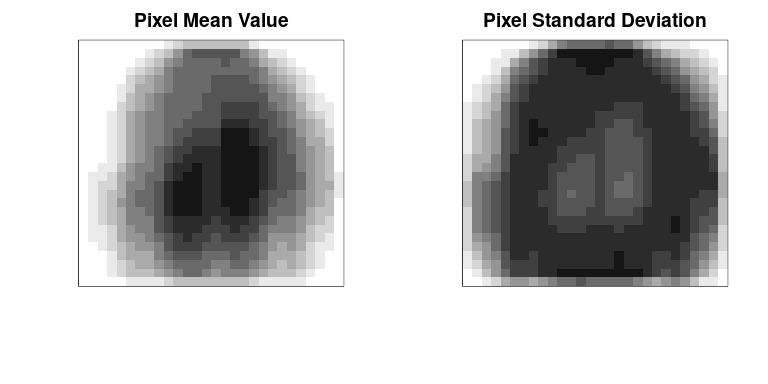
\includegraphics[width=0.9\linewidth]{/home/bonzilla/Documents/MSDS/Data622_group5_projects/FinalReport_Data622/pixvals} 

}

\caption{Pixel values across dataset. Left panel: mean pixel values. Right panel: pixel value standard deviation}\label{fig:unnamed-chunk-2}
\end{figure}

\hypertarget{principal-component-analysis}{%
\section{Principal Component
Analysis}\label{principal-component-analysis}}

\label{sec:headings}

We have shown above that there is redundancy in the fashion MNIST
dataset. Here we will use PCA to reduce the number of features while
retaining as much of the variance possible. PCA does this by finding a
new set of axes that fit to the variance of the data. At heart, PCA is
simply an eigendecomposition of the data which returns a set of
eigenvectors and eigenvalues. Eigenvectors and eigenvalues describe the
transformations necessary to go from the original axes to a new feature
space.

We can use the results of PCA to perform a type of information
compression on the original data by subsetting the amount of PCA
components we use to describe the original data. For this analysis, we
will use a criterion of 95\% variance explained. From the 784 components
that PCA yields, we will subset the minimum components needed such that
the sum of the proportions of explained variance is greater than or
equal to 95\%. Such a manipulation is favorable because it will reduce
redundancy in the data, the chances of overfitting, and the time
necessary to train models.

\begin{figure}

{\centering 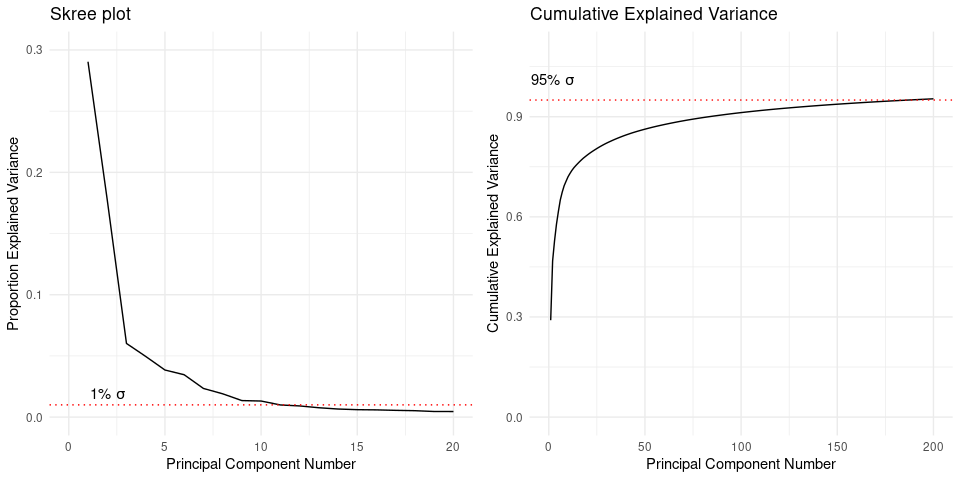
\includegraphics[width=0.9\linewidth]{/home/bonzilla/Documents/MSDS/Data622_group5_projects/FinalReport_Data622/pcaskree} 

}

\caption{PCA Results. The Skree plot (Left) shows the proportion on explained variance for each the first 20 principal components. The Cumulative Explained Variance plot (Right) shows the total variance explained by successively addding up to 200 principal components}\label{fig:unnamed-chunk-3}
\end{figure}

From the skree plot, we can see a very sharp drop off in the proportion
of explained variance. Principal Components greater than 12 account for
less than 1\% of the dataset's variance. The first 12 components only
account for a cumulative variance of 0.74, therefore it takes the
combined contribution of many more components (187 components) to
explain 95\% of the variance of each pixel for the original images.

\begin{figure}

{\centering 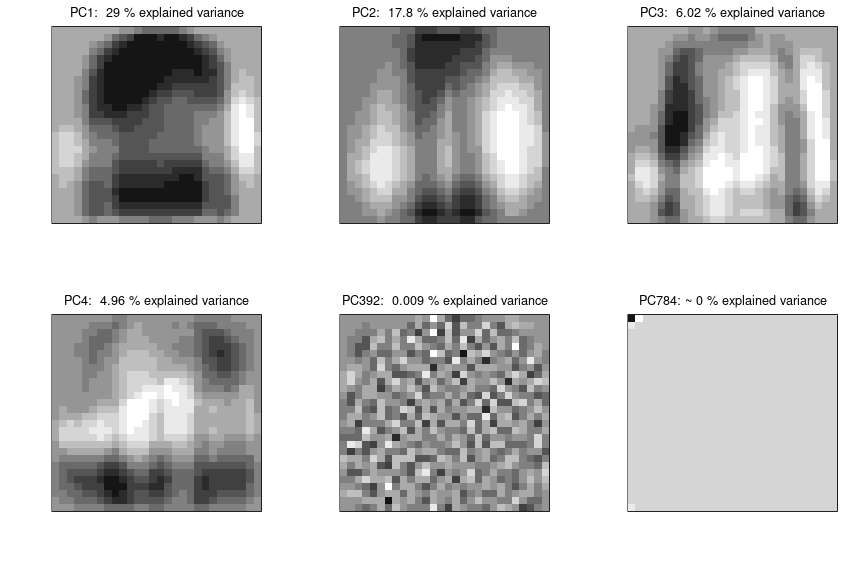
\includegraphics[width=0.9\linewidth]{/home/bonzilla/Documents/MSDS/Data622_group5_projects/FinalReport_Data622/pcacomps} 

}

\caption{Visualizing PCA Components. The top row (from left to right) and bottom left panel visualize principal components 1 through 4. The middle panel of the bottom row shows the 392th component. The bottom right panels shows principal component 784}\label{fig:unnamed-chunk-4}
\end{figure}

PCA returns a components for every dimension of the data in descending
order of the amount of variance accounted for. The figure above shows
the the first 4 components, component PC392 (middle), and the last
component PC784. As already depicted in the Skree and Cumulative
Explained Variance plots, the first four components explain 0.58\%
variance from PC1: 22.1\% \(\rightarrow\) PC2: 5.1\% variance. We can
see clearly from the visualization of the components that the first
several PCs are clearly discriminating between clothing classifications.
For instance, PC1 distinguishes between T-shirt/top \& Pullover
(dark/high values) and shoe categories (light/low values). On the other
hand, PC2 appears to distinguish Trousers from shoe categories. The
representation become less clear as the explained variance decreases.
For instance, PC392 and PC784 only explain 0.01\% and 0.001\% variance
respectively and it is not clear from the visualization just what
information these components represent.

PC1 and PC2 account for roughly half (0.47) of the train dataset's
variance. We can visualize the projections of the train data onto the
features space of these two components:

\begin{figure}

{\centering 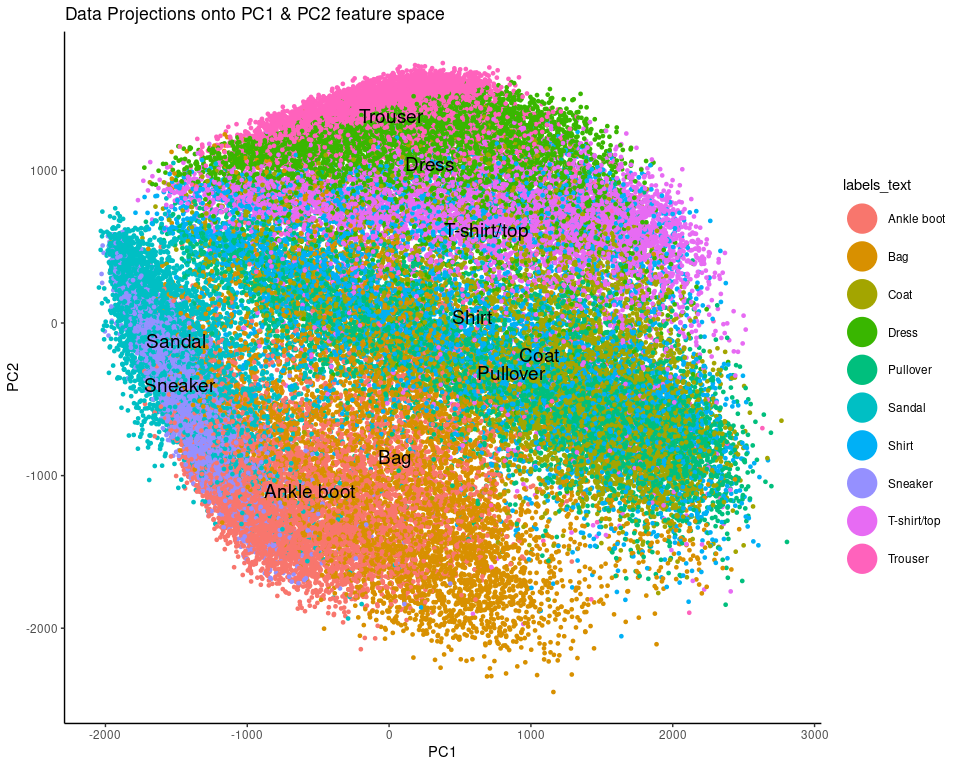
\includegraphics[width=0.9\linewidth]{/home/bonzilla/Documents/MSDS/Data622_group5_projects/FinalReport_Data622/pcaproj} 

}

\caption{Magnitudes of PCA 1 and 2 for all Fashion-MNIST images from the 'train' dataset. Datapoints are shaded according the clothing category. A black text label is rendered at the mean PC1 and PC2 values for each category.}\label{fig:unnamed-chunk-5}
\end{figure}

The figure above shows the representations of the \texttt{train} images
in the feature space of the first 2 dimensions. Each clothing item
category is represented by a different color. For clarity, a text label
(in black) which corresponds to the categorical mean values of PC1 \&
PC2 has been added. We can see that there is noticeable separation
across the categories. Additionally, we see some clustering of category
means that meets expectations. For example, the shoe categories (Sandal,
Sneaker and Ankle Boot) group together towards the lower left hand
corner of the figure. Clothing items that could all be described as tops
with sleeves ( Pullover, Coat, Shirt \& T-shirt/top) group together in
the middle of the distribution. Trousers, on the other hand, have a
noticeable distance from tops with sleeves but ar contiguous with the
dress category which shares roughly vertical rectangular profile.

Here we find the representation onto the first 187 components which were
shown earlier to account for 95\% of the variance in the image data:

\begin{figure}

{\centering 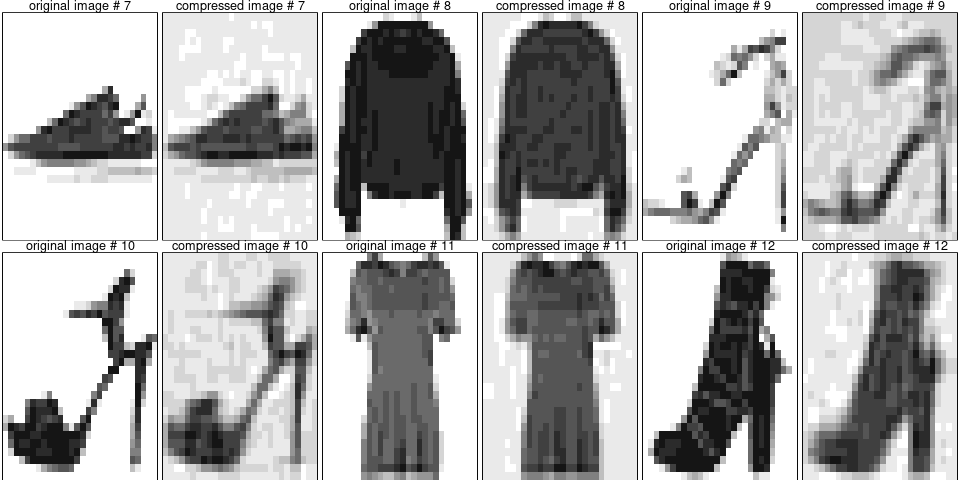
\includegraphics[width=0.9\linewidth]{/home/bonzilla/Documents/MSDS/Data622_group5_projects/FinalReport_Data622/pca_reconstruct} 

}

\caption{Reconstructed Images using 187 Principal Components. Original Fashion-MNIST images are rendered next to the corresponding compressed images which are reconstructed from the first 187 components}\label{fig:unnamed-chunk-6}
\end{figure}

Truncating the data to 187 components does result in information loss,
however, as we can see from the visualizations above, the images retain
much of the detail from the original images while using a feature space
23.85\% the size of the original.

PCA is a dimensionality reduction method that can be applied to high
dimensional datasets. PCA reduces the number of features while
preserving as much variance from the data as possible. Here we used PCA
to reduce the number of features of the Fashion MNIST dataset from 784
to 187. We showed through a series of visualizations that transforming
the images to the reduced feature space does so with an noticeable loss
to image quality, however the gist of the images is still present.

\hypertarget{headings-second-level}{%
\subsection{Headings: second level}\label{headings-second-level}}

\hypertarget{headings-third-level}{%
\subsubsection{Headings: third level}\label{headings-third-level}}

Another paragraph.

\hypertarget{examples-of-citations-figures-tables-references}{%
\section{Examples of citations, figures, tables,
references}\label{examples-of-citations-figures-tables-references}}

\label{sec:others}

You can insert references. Here is some text (Kour and Saabne 2014b,
2014a) and see Hadash et al. (2018).

The documentation for \verb+natbib+ may be found at

You can use custom blocks with LaTeX support from \textbf{rmarkdown} to
create environment.

\begin{center}
\url{http://mirrors.ctan.org/macros/latex/contrib/natbib/natnotes.pdf\%7D}

\end{center}

Of note is the command \verb+\citet+, which produces citations
appropriate for use in inline text.

You can insert LaTeX environment directly too.

\begin{verbatim}
   \citet{hasselmo} investigated\dots
\end{verbatim}

produces

\begin{quote}
  Hasselmo, et al.\ (1995) investigated\dots
\end{quote}

\begin{center}
  \url{https://www.ctan.org/pkg/booktabs}
\end{center}

\hypertarget{figures}{%
\subsection{Figures}\label{figures}}

You can insert figure using LaTeX directly.

See Figure \ref{fig:fig1}. Here is how you add footnotes. {[}\^{}Sample
of the first footnote.{]}

\begin{figure}
  \centering
  \fbox{\rule[-.5cm]{4cm}{4cm} \rule[-.5cm]{4cm}{0cm}}
  \caption{Sample figure caption.}
  \label{fig:fig1}
\end{figure}

But you can also do that using R.

\begin{Shaded}
\begin{Highlighting}[]
\FunctionTok{plot}\NormalTok{(mtcars}\SpecialCharTok{$}\NormalTok{mpg)}
\end{Highlighting}
\end{Shaded}

\begin{figure}
\centering
\includegraphics{FinalReport_Data622_files/figure-latex/fig2-1.pdf}
\caption{Another sample figure}
\end{figure}

You can use \textbf{bookdown} to allow references for Tables and
Figures.

\hypertarget{tables}{%
\subsection{Tables}\label{tables}}

Below we can see how to use tables.

See awesome Table\textasciitilde{}\ref{tab:table} which is written
directly in LaTeX in source Rmd file.

\begin{table}
 \caption{Sample table title}
  \centering
  \begin{tabular}{lll}
    \toprule
    \multicolumn{2}{c}{Part}                   \\
    \cmidrule(r){1-2}
    Name     & Description     & Size ($\mu$m) \\
    \midrule
    Dendrite & Input terminal  & $\sim$100     \\
    Axon     & Output terminal & $\sim$10      \\
    Soma     & Cell body       & up to $10^6$  \\
    \bottomrule
  \end{tabular}
  \label{tab:table}
\end{table}

You can also use R code for that.

\begin{Shaded}
\begin{Highlighting}[]
\NormalTok{knitr}\SpecialCharTok{::}\FunctionTok{kable}\NormalTok{(}\FunctionTok{head}\NormalTok{(mtcars), }\AttributeTok{caption =} \StringTok{"Head of mtcars table"}\NormalTok{)}
\end{Highlighting}
\end{Shaded}

\begin{longtable}[]{@{}lrrrrrrrrrrr@{}}
\caption{Head of mtcars table}\tabularnewline
\toprule
& mpg & cyl & disp & hp & drat & wt & qsec & vs & am & gear &
carb\tabularnewline
\midrule
\endfirsthead
\toprule
& mpg & cyl & disp & hp & drat & wt & qsec & vs & am & gear &
carb\tabularnewline
\midrule
\endhead
Mazda RX4 & 21.0 & 6 & 160 & 110 & 3.90 & 2.620 & 16.46 & 0 & 1 & 4 &
4\tabularnewline
Mazda RX4 Wag & 21.0 & 6 & 160 & 110 & 3.90 & 2.875 & 17.02 & 0 & 1 & 4
& 4\tabularnewline
Datsun 710 & 22.8 & 4 & 108 & 93 & 3.85 & 2.320 & 18.61 & 1 & 1 & 4 &
1\tabularnewline
Hornet 4 Drive & 21.4 & 6 & 258 & 110 & 3.08 & 3.215 & 19.44 & 1 & 0 & 3
& 1\tabularnewline
Hornet Sportabout & 18.7 & 8 & 360 & 175 & 3.15 & 3.440 & 17.02 & 0 & 0
& 3 & 2\tabularnewline
Valiant & 18.1 & 6 & 225 & 105 & 2.76 & 3.460 & 20.22 & 1 & 0 & 3 &
1\tabularnewline
\bottomrule
\end{longtable}

\hypertarget{lists}{%
\subsection{Lists}\label{lists}}

\begin{itemize}
\tightlist
\item
  Item 1
\item
  Item 2
\item
  Item 3
\end{itemize}

In your report, be sure to:

\begin{itemize}
\item
  describe the problem you are trying to solve.
\item
  describe your datasets and what you did to prepare the data for
  analysis.
\item
  methodologies you used for analyzing the data
\item
  why you did what you did
\item
  make your conclusions from your analysis. Please be sure to address
  the business impact (it could be of any domain) of your solution.
\end{itemize}

\hypertarget{refs}{}
\begin{CSLReferences}{1}{0}
\leavevmode\hypertarget{ref-hadash2018estimate}{}%
Hadash, Guy, Einat Kermany, Boaz Carmeli, Ofer Lavi, George Kour, and
Alon Jacovi. 2018. {``Estimate and Replace: A Novel Approach to
Integrating Deep Neural Networks with Existing Applications.''}
\emph{arXiv Preprint arXiv:1804.09028}.

\leavevmode\hypertarget{ref-kour2014fast}{}%
Kour, George, and Raid Saabne. 2014a. {``Fast Classification of
Handwritten on-Line Arabic Characters.''} In \emph{Soft Computing and
Pattern Recognition (SoCPaR), 2014 6th International Conference of},
312--18. IEEE.

\leavevmode\hypertarget{ref-kour2014real}{}%
---------. 2014b. {``Real-Time Segmentation of on-Line Handwritten
Arabic Script.''} In \emph{Frontiers in Handwriting Recognition (ICFHR),
2014 14th International Conference on}, 417--22. IEEE.

\leavevmode\hypertarget{ref-krizhevsky2009learning}{}%
Krizhevsky, Alex, Geoffrey Hinton, and others. 2009. {``Learning
Multiple Layers of Features from Tiny Images.''}

\leavevmode\hypertarget{ref-lecun1998gradient}{}%
LeCun, Yann, Léon Bottou, Yoshua Bengio, and Patrick Haffner. 1998.
{``Gradient-Based Learning Applied to Document Recognition.''}
\emph{Proceedings of the IEEE} 86 (11): 2278--2324.

\leavevmode\hypertarget{ref-noever2021overhead}{}%
Noever, David, and Samantha E Miller Noever. 2021. {``Overhead Mnist: A
Benchmark Satellite Dataset.''} \emph{arXiv Preprint arXiv:2102.04266}.

\leavevmode\hypertarget{ref-xiao2017fashion}{}%
Xiao, Han, Kashif Rasul, and Roland Vollgraf. 2017. {``Fashion-Mnist: A
Novel Image Dataset for Benchmarking Machine Learning Algorithms.''}
\emph{arXiv Preprint arXiv:1708.07747}.

\end{CSLReferences}

\bibliographystyle{unsrt}
\bibliography{references.bib}


\end{document}
